\documentclass[12pt,aspectratio=169]{beamer}

\usetheme[
    sectionpage=progressbar,
    subsectionpage=progressbar,
    progressbar=frametitle
]{metropolis}

\usefonttheme{professionalfonts}

\definecolor{blue-grey-900}{HTML}{263238}
\definecolor{deep-orange-500}{HTML}{FF5722}
\setbeamercolor{normal text}{fg=blue-grey-900, bg=white}
\setbeamercolor{alerted text}{fg=deep-orange-500}

\usepackage{booktabs}
\usepackage{graphicx}
\usepackage{hyphenat}
\usepackage{multirow}

\usepackage{polyglossia}
\setdefaultlanguage[variant=british]{english}
\usepackage[english=british]{csquotes}

\usepackage{fontspec}
\setmainfont{Lucida Sans OT}
\setsansfont[Scale=MatchLowercase]{Lucida Sans OT}
\setmonofont[Scale=MatchLowercase]{Lucida Console DK}
\defaultfontfeatures{Ligatures=TeX}

\usepackage{mathspec}
\setmathsfont(Digits,Latin,Greek)[Numbers={Lining,Proportional}]{Lucida Bright Math OT}

\author{Gianluca Campanella}
\title{Data Science for Scientists}
\date{17\textsuperscript{th} July 2018}



\subtitle{The Data Science process}

\begin{document}

\maketitle

\begin{frame}{High\hyp{}level view}
    \only<1>{%
        \begin{center}
            \large%
            Business goal
            \vfill
            $\downarrow$
            \vfill
            Testable hypothesis
            \vfill
            $\downarrow$
            \vfill
            Experimentation and modelling
        \end{center}}
    \only<2>{%
        \begin{center}
            \large%
            Research question
            \vfill
            $\downarrow$
            \vfill
            Obtain $\ \longleftrightarrow\ $ Explore $\ \longleftrightarrow\ $ Model
            \vfill
            $\downarrow$
            \vfill
            \textbf{Use it!}
        \end{center}}
\end{frame}

\begin{frame}
    \begin{center}
        \LARGE%
        Which takes longer?
    \end{center}
\end{frame}

\begin{frame}
    \large%
    \begin{quote}
        What people think of as the moment of discovery is really the discovery
        of the question.

        \begin{flushright}
            --- J.\ E.\ Salk
        \end{flushright}
    \end{quote}
\end{frame}

\begin{frame}[t]{Define the research question}
    \begin{block}{What to do}
        \begin{itemize}
            \item Identify the problem and why it should be solved
            \item Frame it in the context of data collection
        \end{itemize}
    \end{block}
    \vfill\pause
    \begin{block}{What to ask}
        \begin{itemize}
            \item Which metrics do I need to improve?
            \item What are possible actions to solve the problem?
            \item What is the benefit of solving the problem?
        \end{itemize}
    \end{block}
\end{frame}

\begin{frame}[t]{Obtain the data}
    \begin{block}{What to do}
        \begin{itemize}
            \item Measure the gap between ideal and available
            \item Think about assumptions and limitations
        \end{itemize}
    \end{block}
    \vfill\pause
    \begin{block}{What to ask}
        \begin{itemize}
            \item Are there enough data?
            \item Are they relevant to the research question?
            \item Can they be trusted?
        \end{itemize}
    \end{block}
\end{frame}

\begin{frame}[t]{Explore the data}
    \begin{block}{What to do}
        \begin{itemize}
            \item Data dictionary and any other documentation
            \item Descriptive statistics and visualisations
        \end{itemize}
    \end{block}
    \vfill\pause
    \begin{block}{What to ask}
        \begin{itemize}
            \item What kind of simple visualisations can I use?
            \item Which data types and distributions?
            \item Are there missing values or outliers?
        \end{itemize}
    \end{block}
\end{frame}

\begin{frame}[t]{Model the data}
    \begin{block}{What to do}
        \begin{itemize}
            \item Model selection and fitting
            \item Feature engineering
        \end{itemize}
    \end{block}
    \vfill\pause
    \begin{block}{What to ask}
        \begin{itemize}
            \item Analysis\hyp{}focused or building\hyp{}focused?
            \item What is an appropriate model for the data?
            \item How can I evaluate and improve model performance?
        \end{itemize}
    \end{block}
\end{frame}

\begin{frame}{Modelling misconceptions}
    Most well\hyp{}executed Data Science projects don't\ldots
    \begin{itemize}
        \item Use complicated tools
        \item Fit complicated models
    \end{itemize}
    \vfill\pause
    Instead, they do\ldots
    \begin{itemize}
        \item Focus on solving the problem
        \item Use appropriate --- not necessarily big! --- data
        \item Use relatively standard models
    \end{itemize}
\end{frame}

{\setbeamertemplate{background}{%
    \rule{0.7\paperwidth}{0pt}%
    \rule{0pt}{\paperheight}%
    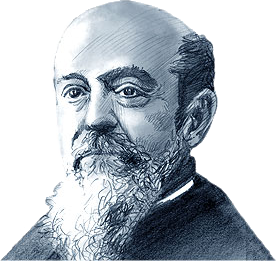
\includegraphics[height=0.6\paperheight]{figures/pareto}}
\begin{frame}{The 80---20 rule of modelling}
    \begin{itemize}
        \item The first reasonable thing you can do goes 80\% of the way
        \item Everything after that is to get the remaining 20\%\ldots \\
              often at additional cost!
    \end{itemize}
    \vfill\pause
    \begin{center}
        \Large%
        Is it worth it?
    \end{center}
\end{frame}}

\begin{frame}
    \begin{center}
        \LARGE%
        Are we done?
    \end{center}
\end{frame}

\begin{frame}[t]{Summarise the findings}
    \begin{block}{What to do}
        \begin{itemize}
            \item Storytelling and visual aids to interpretation
            \item Communicate assumptions and limitations
        \end{itemize}
    \end{block}
    \vfill\pause
    \begin{block}{What to ask}
        \begin{itemize}
            \item How can I communicate results effectively?
            \item What format should I adopt?
            \item Who are my audience?
        \end{itemize}
    \end{block}
\end{frame}

\begin{frame}[t]{Operationalise}
    \begin{block}{What to do}
        \begin{itemize}
            \item System integration
            \item Monitoring and maintenance
        \end{itemize}
    \end{block}
    \vfill\pause
    \begin{block}{What to ask}
        \begin{itemize}
            \item What (visual) outputs do I care about?
            \item How often does the model need retraining?
            \item Do we need to think about scalability?
        \end{itemize}
    \end{block}
\end{frame}

\begin{frame}{Caveat}
    \begin{center}
        \Large%
        This process is \\
        non\hyp{}linear and iterative
    \end{center}
\end{frame}

\end{document}

